\documentclass[tikz,border=2pt]{standalone}
\usepackage{amsmath}
\usepackage{pgfplots}
\pgfplotsset{compat=1.18}

\begin{document}
% Ratio test on a_n = n/2^n: the ratios a_{n+1}/a_n = (n+1)/(2n) tend to L = 1/2 < 1, so from
% n = 3 on each term is at most 2/3 of the previous one and the terms sit under a geometric
% series — the series converges.
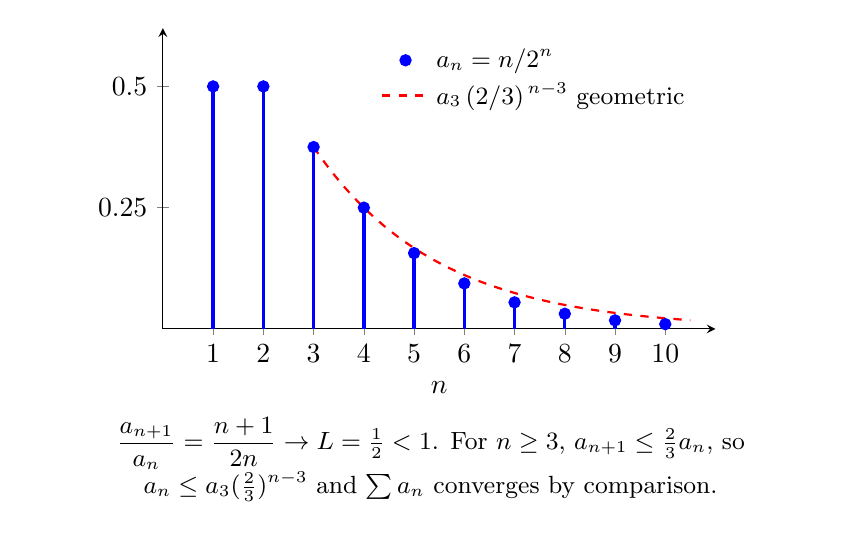
\begin{tikzpicture}
	\begin{axis}[
		axis lines=left,
		xmin=0, xmax=11, ymin=0, ymax=0.62,
		xtick={1,...,10}, ytick={0.25,0.5},
		xlabel={$n$},
		width=8.6cm, height=5.4cm, clip=false,
		legend pos=north east, legend style={draw=none, fill=none, font=\small}, legend cell align=left
		]
		\addplot[ycomb, blue, very thick, mark=*, mark size=1.6pt] coordinates {(1,0.5) (2,0.5) (3,0.375) (4,0.25) (5,0.15625) (6,0.09375) (7,0.0547) (8,0.03125) (9,0.01758) (10,0.00977)};
		\addlegendentry{$a_n=n/2^n$}
		\addplot[red, thick, dashed, domain=3:10.5, samples=60] {0.375*(2/3)^(x-3)};
		\addlegendentry{$a_3\,(2/3)^{\,n-3}$ geometric}
	\end{axis}
	\node[anchor=north, align=flush center, text width=10cm, font=\small] at (3.4,-1.0) {$\dfrac{a_{n+1}}{a_n}=\dfrac{n+1}{2n}\to L=\tfrac12<1$. For $n\ge3$, $a_{n+1}\le\tfrac23a_n$, so $a_n\le a_3(\tfrac23)^{n-3}$ and $\sum a_n$ converges by comparison.};
\end{tikzpicture}
\end{document}
